\begin{figure*}[hb]
    \centering 
    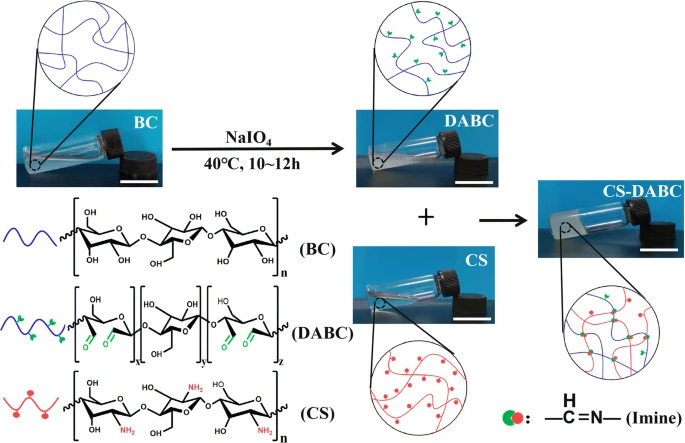
\includegraphics[width=0.7\linewidth]{Figures/CS_DABC_condensation.jpg}
    \caption{Schematic representation of hydrogel synthesis from chitosan and dialdehyde bacterial cellulose \autocite{liAllnaturalInjectableHydrogel2020}}
    \label{fig:CS_DABC_condensation}
\end{figure*}

A recent study by \citeauthor{liAllnaturalInjectableHydrogel2020} found that an all-natural, injectable hydrogel could be synthesized using chitosan and dialdehyde bacterial cellulose (\citeyear{liAllnaturalInjectableHydrogel2020}). This hydrogel uses imine bond dynamic cross-linkages to achieve its self-healing properties, where the Schiff base forms through the reaction of chitosan (as the amine) and bacterial cellulose (as the aldehyde).
The reaction can proceed under mild conditions (room temperature and pH = 7.2), and as it is all-natural, it has shown to be biocompatible. A schematic representation of this condensation reaction is given in Figure~\ref{fig:CS_DABC_condensation}.

Additionally, the chitosan dressing exhibits antimicrobial properties, which reduces the risk of cross-contamination and promotes healthy healing of the wound.
This self-healing hydrogel presents a promising application for tendon repair. Since JTAs already have a chitosan layer, it could be possible to synthesize Schiff bases directly on the existing structure using a similar technique as \citeauthor{liAllnaturalInjectableHydrogel2020}, leading to increased mechanical strength through the integration of self-healing properties.
% This self-healing hydrogel, therefore, has an interesting application for tendon repair. Given that JTAs have a chitosan side, it could be possible to augment their mechanical strength by integrating self-healing properties.